\documentclass[a4paper, openany]{memoir}

\usepackage[utf8]{inputenc}
\usepackage[T1]{fontenc} 
\usepackage[english]{babel}
\usepackage{amsmath}
\usepackage{amssymb}
\usepackage{amsthm}

\usepackage{booktabs}
\usepackage{fancyhdr}
\usepackage{float}
\usepackage{indentfirst}
\usepackage{graphicx}
\usepackage[linewidth=1pt]{mdframed}
\usepackage{multicol}
\usepackage{fancyvrb}
\usepackage{tikz}

\newcommand{\nfrac}[2]{
    {\displaystyle\frac{#1}{\strut #2}}
  \kern-\nulldelimiterspace}

\pagestyle{fancy}
\fancyhf{}
\fancyhead[LE]{\leftmark}
\fancyhead[RO]{\rightmark}
\fancyhead[RE, LO]{ToC}
\fancyfoot[LE, RO]{\thepage}
\fancyfoot[RE, LO]{Pete Gautam}

\renewcommand{\headrulewidth}{1.5pt}

\newtheorem{proposition}{Proposition}[section]
\newtheorem{lemma}[proposition]{Lemma}
\newtheorem{theorem}[proposition]{Theorem}
\newtheorem{corollary}[proposition]{Corollary}

\theoremstyle{definition}
\newtheorem{definition}[proposition]{Definition}

\chapterstyle{thatcher}

\begin{document}
    \chapter{Lambda Calculus}
    \section{Introduction to Lambda Calculus}
    In this section, we will study the syntax and the semantics of \emph{Lambda Calculus}, along with some of its properties. Lambda Calculus (denoted $\lambda$-calculus) is a mathematical theory of \emph{functions}, including:
    \begin{itemize}
        \item a formal syntax for defining functions;
        \item a formal semantics of how functions can be evaluated; and
        \item a formal theory of function equivalence.
    \end{itemize}

    We first define the syntax of $\lambda$-calculus. We denote by the set $\Lambda$ the set of all $\lambda$-terms. It is the \emph{smallest} set satisfying the following properties:
    \begin{itemize}
        \item If $x$ is a \emph{variable}, then $x \in \Lambda$ (i.e. there are infinitely many variables);
        \item If $M \in \Lambda$, then the \emph{abstraction} $(\lambda x M) \in \Lambda$;
        \item If $M, N \in \Lambda$, then the \emph{application} $(MN) \in \Lambda$.
    \end{itemize}
    This is an inductive definition for $\Lambda$. An abstraction represents a function, e.g. the $\lambda$-term $(\lambda x x)$ can be thought of as the Haskell function $\backslash \texttt{x -> x}$. 
    
    We can define $\lambda$-calculus using BNF as well:
    \begin{align*}
        M &::= x \\
        &| \ (\lambda x M) \\
        &| \ (MM)
    \end{align*}
    Note that in the last line, although we have the application $(MM)$, the two $M$ values need not be the same. Further, we can use inference rules to define it:
    \[\frac{\textrm{if } x \textrm{ is a variable}^*}{x \in \Lambda} \qquad \frac{M \in \Lambda \textrm{ and } x \textrm{ is a variable}^*}{(\lambda x M) \in \Lambda} \qquad \frac{M, N \in \Lambda}{(MN) \in \Lambda}.\]

    We typically avoid using brackets for $\lambda$-terms. Moreover, an abstraction $(\lambda x M)$ is denoted $\lambda x.M$. If we have multiple abstractions, we write
    \[\lambda x_1 \dots x_k . M \equiv \lambda \vec{x}. M \equiv (\lambda x_1 (\dots (\lambda x_k M) \dots ))\]
    The symbol $\equiv$ denotes syntactic equivalence. Note that abstraction is \emph{right-associative}. Now, if we have multiple applications, we write
    \[M N_1 \dots N_k \equiv M \vec{N} \equiv (((M N_1) \dots ) N_k)\]
    Note that application is \emph{left-associative}.

    \subsection{Free and Bound Variables}
    The symbol $\lambda$ is a \emph{variable binder}, i.e. it gives rise to local variables. As such, different terms are equivalent, e.g. $\lambda x. x$ and $\lambda y. y$. Moreover, this gives rise to \emph{free variables} (not bound by $\lambda$) and \emph{bound variables} (those bound by $\lambda$).

    We will now define the set of bound variables formally. It is a function $BV \colon \Lambda \to \mathcal{P}(\textit{Var})$, where $\textit{Var}$ is the set of variables, and $\mathcal{P}(\textit{Var})$ is the set of all subsets of variables. It is defined recursively:
    \begin{align*}
        BV \ x &= \varnothing \\
        BV \ \lambda x. M &= (BV \ M) \cup \{x\} \\
        BV \ MN &= (BV \ M) \cup (BV \ N)
    \end{align*}
    We illustrate this with an example. Consider the term $(\lambda y. (\lambda x. zx)) y$. Then, we compute its bound variables as follows:
    \begin{align*}
        BV \ (\lambda y. (\lambda x. zx)) y &= (BV \ \lambda y. (\lambda x. zx)) \cup (BV \ y) \\
        &= ((BV \ \lambda x.zx) \cup \{y\}) \cup \varnothing \\
        &= (((BV \ zx) \cup \{x\}) \cup \{y\}) \\
        &= ((BV \ z) \cup (BV \ x)) \cup \{x, y\} \\
        &= \varnothing \cup \varnothing \cup \{x, y\} \\
        &= \{x, y\}.
    \end{align*}

    Next, we define free variables. It too is a function $FV \colon \Lambda \to \mathcal{P}(\textit{Var})$, given by:
    \begin{align*}
        FV \ x &= \{x\} \\
        FV \ \lambda x. M &= (FV \ M) \setminus \{x\} \\
        FV \ MN &= (FV \ M) \cup (FV \ N)
    \end{align*}
    We illustrate this with an example:
    \begin{align*}
        FV \ (\lambda y. (\lambda x. zx)) y &= (FV \ \lambda y.(\lambda x. zx)) \cup (FV \ y) \\
        &= ((FV \ \lambda x.xz) \setminus \{y\}) \cup \{y\} \\
        &= ((FV \ xz \setminus \{x\}) \setminus \{y\}) \cup \{y\} \\
        &= (((FV \ x) \cup (FV \ z) \setminus \{x, y\})) \cup \{y\} \\
        &= (\{x, z\} \setminus \{x, y\}) \cup \{y\} \\
        &= \{y, z\}.
    \end{align*}

    We now define \emph{subterms} of a term. It is a function $Sub \colon \Lambda \to \mathcal{P}(\Lambda)$ defined by:
    \begin{align*}
        Sub \ x &= \{x\} \\
        Sub \ \lambda x. M &= (Sub \ M) \cup \{\lambda x. M\} \\
        Sub \ MN &= (Sub \ M) \cup (Sub \ N) \cup \{MN\}
    \end{align*}
    We illustrate this with an example:
    \begin{align*}
        Sub \ (\lambda y. (\lambda x. zx)) y &= (Sub \ \lambda y. (\lambda x. zx)) \cup (Sub \ y) \cup \{(\lambda y. (\lambda x. zx)) y\} \\
        &= (Sub \ \lambda x. zx \cup \{\lambda y. (\lambda x. zx)\}) \cup \{y, (\lambda y. (\lambda x. zx)) y\} \\
        &= ((Sub \ zx) \cup \{\lambda x. zx\}) \cup \{\lambda y. (\lambda x. zx), y, (\lambda y. (\lambda x. zx)) y\} \\
        &= ((Sub \ z) \cup (Sub \ x) \cup \{zx\}) \cup \\
        &\hspace*{12pt} \{\lambda x. zx, \lambda y. (\lambda x. zx), y, (\lambda y. (\lambda x. zx)) y\} \\
        &= \{z\} \cup \{x\} \cup \{zx, \lambda x. zx, \lambda y. (\lambda x. zx), y, (\lambda y. (\lambda x. zx)) y\}  \\
        &= \{z, x, zx, \lambda x. zx, \lambda y. (\lambda x. zx), y, (\lambda y. (\lambda x. zx)) y\}.
    \end{align*}

    \subsection{Structural Induction}
    We will now look at proofs involving structural induction for $\lambda$-calculus. We start wth an easy example.
    \begin{proposition}
        A term in $\Lambda$ has balanced parentheses.
    \end{proposition}
    \begin{proof}
        We show that using structural induction on a term:
        \begin{itemize}
            \item In the base case, the term is $x$, for some variable $x$. Since there are no parentheses here, the result follows trivially.
            \item Now, assume that the terms $M$ and $N$ have balanced parentheses. Then, the term $(MN)$ must also have balanced parentheses.
            \item Finally, assume that the term $M$ has balanced parentheses. Then, the term $(\lambda x M)$ must also have balanced parentheses.
        \end{itemize}
        So, the result follows by structural induction.
    \end{proof}
    \noindent Note that we have 2 inductive cases here- this is because there are 3 production rules. We now look at a more complicated example.
    \begin{proposition}
        Let $M$ be a term. Then, $FV \ M \subseteq Sub \ M$.
    \end{proposition}
    \begin{proof}
        We prove this by structural induction on $M$.
        \begin{itemize}
            \item In the base case, we have $M = x$, for some variable $x$. Then,
            \[FV \ M = \{x\} \subseteq \{x\} = Sub \ M.\]

            \item Now, assume that $M = N_1 N_2$, for terms $N_1$ and $N_2$. By the inductive hypothesis, we know that $FV \ N_1 \subseteq Sub \ N_1$ and $FV \ N_2 \subseteq Sub \ N_2$. Hence,
            \begin{align*}
                FV \ M &= (FV \ N_1) \cup (FV \ N_2) \\
                &\subseteq (Sub \ N_1) \cup (Sub \ N_2) \\
                &\subseteq (Sub \ N_1) \cup (Sub \ N_2) \cup \{M\} = Sub \ M.
            \end{align*}

            \item Finally, assume that $M = \lambda x. N$, for some term $N$. By the inductive hypothesis, $FV \ N \subseteq Sub \ N$. Then,
            \begin{align*}
                FV \ M &= (FV \ N) \setminus \{x\} \\
                &\subseteq FV \ N \\
                &\subseteq Sub \ N \\
                &\subseteq (Sub \ N) \cup \{M\} = Sub \ M.
            \end{align*}
        \end{itemize}
        So, the result follows from structural induction.
    \end{proof}

    \subsection{Contexts}
    A \emph{context} is a term containing a \emph{hole}, which is represented by $[]$. This hole can be filled by a term, to make the context a term. It is defined as follows:
    \begin{align*}
        C[] &::= x \\
        &| \ [] \\
        &| \ (\lambda x C[]) \\
        &| \ (C[] C[])
    \end{align*}
    The variable has no hole; the empty context is $[]$. The context $C[] C'[]$ has two holes. 
    
    We will now illustrate how to fill a context with a term. So, consider the context 
    \[C[] = ((\lambda x. [] x) M).\]
    Then, 
    \[C[\lambda y.y] = ((\lambda x.(\lambda y.y) x) M).\]
    We have replaced the hole $[]$ with the given term.

    In general, we can fill contexts with a hole given one term.
    \begin{proposition}
        Let $C[]$ be a context with one hole and $M$ a term. Then, $C[M]$ is a term.
    \end{proposition}
    \begin{proof}
        We show this using structural induction on the context $C[]$.
        \begin{itemize}
            \item First, let $C[] = []$. Since $M$ is a term, we find that $C[M] = M$ is a term.
            \item Now, let $C[] = \lambda x. C'[]$, where $C'[]$ is a context where $C'[M]$ is a term. Then, $C[M] = \lambda x. C'[M]$ must be a term.
        \end{itemize}
        So, the result follows from structural induction.
    \end{proof}
    \noindent Note that we only considered 2 of the cases from the definition of a context- a variable $x$ has no holes, while the context $(C[] C[])$ has two.
    
    In general, we can fill a context with $n$ holes given $n$ terms- this follows from the result above and mathematical induction.

    \newpage

    \section{Reduction}
    In this section, we will consider how we can evaluate $\lambda$-terms, using the $\beta$-rule in a cumbersome manner, and later using $\beta$-rule with $\alpha$-equivalence to make it compact and efficient.

    \subsection{$\beta$-reduction}
    The key definition for expressing computation in $\lambda$-calculus is the $\beta$-rule. It states:
    \[(\lambda x. M) N \to_\beta M[x := N]\]
    The notation $M[x := N]$ refers to substitution- every occurrence of $x$ in $M$ is replaced by $N$. For example,
    \[(\lambda x. x+1) 2 \to_\beta (x + 1)[x := 2] \equiv 2 + 1.\]
    We could further reduce this to $3$ by extending mathematical operations, like in the language \textit{Expr}. The $\beta$-rule expresses how we would like to pass parameters into a function.

    Substitution is the main aspect of $\beta$-reduction. However, naive substitution is not necessarily what we want in general. For instance, if we have the term $(\lambda x.\lambda y.yx) y$, then we can $\beta$-reduce it to $\lambda y. yy$. However, this is not what we would like- the first $y$ is meant to be bound by the local $y$, but the second one is not- it is the value we have just substituted. This would not have happened if we have the term $(\lambda x. \lambda y. yx)z$, in which case we get $\lambda y.yz$. So, this happens in the term $(\lambda x. \lambda y. yx)y$ because $y$ is both a free and a bound variable in the term.

    Hence, we need to define substitution in a more careful manner. This is done as follows:
    \begin{enumerate}
        \item $x[x := N] \equiv N$;
        \item $y[x := N] \equiv y$ if $x$ and $y$ are distinct;
        \item $(\lambda x.M)[x := N] \equiv \lambda x.M$;
        \item $(\lambda y.M)[x := N] \equiv \lambda y. M[x := N]$ if $x$ is not a free variable in $M$ or $y$ is not a free variable in $N$;
        \item $(\lambda y.M)[x := N] \equiv (\lambda z.M[y:=z])[x := N]$ if $x$ is a free variable in $M$ and $y$ a free variable in $N$, and $z$ is a new variable;
        \item $(M_1 M_2)[x := N] \equiv (M_1[x := N])(M_2[x := N])$.
    \end{enumerate}
    In this definition, we are renaming bound variables if they are also free (at step 5). This is to avoid \emph{variable capture}.
    
    We illustrate the definition with an example. So, consider the term $(\lambda x.\lambda y.yx)y$. This $\beta$-reduces to
    \[(\lambda y.yx)[x := y].\]
    The variable $x$ is free in $\lambda y.yx$ and the variable $y$ is free in $y$. Hence, we apply rule 5 to get
    \[(\lambda y.yx)[x := y] \equiv (\lambda z.yx[y := z])[x := y].\]
    We have $yx[y := z] \equiv zx$ by rules 6 and 1, so
    \[(\lambda z.yx[y := z])[x := y] \equiv (\lambda z.zx)[x := y].\]
    Now, although $x$ is free in $\lambda z.zx$, $z$ is not free in $y$, so we apply step 4 and get
    \[\lambda z.zy\]
    In programming language terms, this is similar to renaming a local variable so that it does not override a global variable.
    
    \subsection{$\alpha$-equivalence}
    We will now give another, simpler, definition for substitution. This works by assuming that bound variables have been renamed so that they are different from any free variables. This ensures that variables cannot be captured. This is called \emph{Barendregt convention} or \emph{variable convention}. To do so, we need define $\alpha$-equivalence.
    \begin{definition}
        Let $M$ and $M'$ be terms. We say that $M'$ is produced by $M$ by a \emph{change of bound variables} if $M \equiv C[\lambda x.N]$ and $M' \equiv C[\lambda y.N[x := y]]$, where $y$ does not occur in $N$, and $C[]$ is a context with one hole.
    \end{definition}
    \noindent Note that filling a hole in a context is different to substitution- we do not care about variable capture when doing so, unlike in substitution. For instance, if $C[] \equiv \lambda x.x[]$, then $C[x] \equiv \lambda x.xx$, even though substitution would have resulted in a variable change.
    \begin{definition}
        Let $M$ and $N$ be terms. We say that $M$ is \emph{$\alpha$-equivalent} to $N$ if $N$ is produced from $M$ by a series of changes of bound variable.
    \end{definition}
    \noindent We use the symbol $\equiv_\alpha$ to denote $\alpha$ equivalence. 
    
    We illustrate $\alpha$-equvalence with an example. We claim that $\lambda x.xy \equiv_\alpha \lambda z.zy$. To see this, let $C[] = []y$, and then 
    \[C[\lambda x.x] \equiv \lambda x.xy \qquad \textrm{and} \qquad C[\lambda z.x[x := z]] \equiv C[\lambda z.z] \equiv \lambda z.zy.\] 
    However, $\lambda x.xy$ is not $\alpha$-equivalent to $\lambda x.xx$. We consider $\alpha$-equivalent terms to be the same as each other.

    From now, we will assume that the terms obey variable convention, i.e. all bound variables are different from each other and from all free variables. If this is not the case, we can achieve this using $\alpha$-equivalence. With this convention, the definition of substitution simplifies to the following:
    \begin{enumerate}
        \item $x[x := N] \equiv N$;
        \item $y[x := N] \equiv y$ if $y$ and $x$ are distinct;
        \item $(\lambda y.M)[x := N] \equiv \lambda y.(M[x := N])$;
        \item $(M_1 M_2)[x := N] \equiv M_1[x := N] M_2[x := N]$.
    \end{enumerate}

    We now consider how substitution interacts with two variables.
    \begin{lemma}[Substitution Lemma]
        Let $M$ and $N$ be terms, and $x, y$ distinct variables with $x$ not free in $L$. Then,
        \[M[x := N][y := L] \equiv M[y := L][x := N[y := L]].\]
    \end{lemma}
    \begin{proof}
        We prove this by structural induction on $M$:
        \begin{itemize}
            \item Let $M = z$, where $z$ is a variable distinct to both $x$ and $y$. In that case,
            \begin{align*}
                M[x := N][y := L] &\equiv z[x := N][y := L] \\
                &\equiv z[y := L] \equiv z,
            \end{align*}
            and
            \begin{align*}
                M[y:= L][x := N[y := L]] &\equiv z[y:= L][x := N[y := L]] \\
                &\equiv z[x := N[y := L]] \equiv z.
            \end{align*}
            So, the result holds in this case.
            
            \item Now, let $M = x$. Then, 
            \begin{align*}
                M[x := N][y := L] &\equiv x[x := N][y := L] \\
                &\equiv N[y := L],
            \end{align*}
            and, since $x$ is not free in $L$,
            \begin{align*}
                M[y:= L][x := N[y := L]] &\equiv x[y:= L][x := N[y := L]] \\
                &\equiv x[x := N[y := L]] \equiv N[y := L].
            \end{align*}
            So, the result holds in this case.

            \item Next, let $M = y$. Then,
            \[M[x := N][y := L] \equiv y[x := N][y := L] \equiv y[y := L] \equiv L,\]
            and, since $x$ is not free in $L$,
            \[M[y := L][x := N[y := L]] \equiv L[x := N[y := L]] \equiv L.\]
            So, the result holds in this case.

            \item Next, let $M = \lambda z.M'$, where $z$ is distinct from $x$ and $y$ and 
            \[M'[x := N][y := L] \equiv M'[y := L][x := N[y := L]].\]
            Then,
            \begin{align*}
                M[x := N][y := L] &\equiv (\lambda z.M')[x := N][y := L] \\
                &\equiv (\lambda z.M'[x := N])[y := L] \\
                &\equiv (\lambda z.M'[x := N][y := L]) \\
                &\equiv (\lambda z.M'[y := L][x := N[y := L]]) \\
                &\equiv (\lambda z.M'[y := L])[x := N[y := L]] \\
                &\equiv (\lambda z.M')[y := L][x := N[y := L]] \\
                &\equiv M[y := L][x := N[y := L]].
            \end{align*}
            So, the result holds in this case.

            \item Finally, let $M = M_1 M_2$, where
            \begin{align*}
                M_1[x := N][y := L] \equiv M_1[y := L][x := N[y := L]] \\
                M_2[x := N][y := L] \equiv M_2[y := L][x := N[y := L]].
            \end{align*}
            Then,
            \begin{align*}
                M[x := N][y := L] &\equiv (M_1 M_2)[x := N][y := L] \\
                &\equiv (M_1 [x := N][y := L]) (M_2[x := N][y := L]) \\
                &\equiv (M_1[y := L][x := N[y := L]]) \\
                &\hspace*{12pt} (M_2[y := L][x := N[y := L]]) \\
                &\equiv (M_1 M_2) [y := L][x := N[y := L]] \\
                &\equiv M[y := L][x := N[y := L]].
            \end{align*}
            So, the result holds in this case.
        \end{itemize}
        Hence, the result follows from induction.
    \end{proof}

    We can now complete the definition on evaluating $\lambda$-terms. First, we define \emph{one-step $\beta$-reduction} $\to_\beta$ by the following inference rules:
    \begin{align*}
        & \frac{}{(\lambda x.M)N \to_\beta M[x := N]} & \frac{M \to_\beta N}{MZ \to_\beta NZ} \\
        & \frac{M \to_\beta N}{ZM \to_\beta ZN} & \frac{M \to_\beta N}{\lambda x.M \to_\beta \lambda x.N}
    \end{align*}
    We have seen the first definition before. The other three allow us to apply the $\beta$-rule in larger terms.

    We can define the \emph{$\beta$-reduction}, denoted by $\twoheadrightarrow_\beta$ that is the \emph{reflexive and transitive closure} of one-step $\beta$-reduction. So, the $\beta$-reduction allows for zero or more $\beta$-step reductions. This is defined by the following inference rules:
    \begin{align*}
        \frac{}{M \twoheadrightarrow_\beta M} && \frac{M \to_\beta N}{M \twoheadrightarrow_\beta N} && \frac{M \twoheadrightarrow_\beta N \quad N \twoheadrightarrow_\beta L}{M \twoheadrightarrow_\beta L}.
    \end{align*}

    It turns out that this definition also extends to contexts.
    \begin{proposition}
        Let $C[]$ be a context with one hole. If $M \to_\beta N$, then $C[M] \to_\beta C[N]$.
    \end{proposition}
    \begin{proof}
        We prove this by structural induction on the context $C[]$:
        \begin{itemize}
            \item First, let $C[] = []$. In that case, if $M \to_\beta N$, then $C[M] = M \to_\beta N = C[N]$.
            \item Now, let $C[] = \lambda x.C'[]$, where $C'[]$ is another context. By the inductive hypothesis, we know that $C'[M] \to_\beta C'[N]$. In that case, applying rule 4 of $\to_\beta$, we find that $C[M] = \lambda x.C'[M] \to \lambda x.C'[N] = C[N]$.
        \end{itemize}
        So, the result follows from induction.
    \end{proof}
    \begin{proposition}
        Let $C[]$ be a context with one hole.  If $M \twoheadrightarrow_\beta N$, then $C[M] \twoheadrightarrow_\beta C[N]$.
    \end{proposition}
    \begin{proof}
        We prove this by structural induction on $\twoheadrightarrow_\beta$:
        \begin{itemize}
            \item If $M \equiv N$, then $C[M] \equiv C[N]$. Hence, $C[M] \twoheadrightarrow_\beta C[N]$.
            \item Instead, if $M \to_\beta N$, then by the result above, we have $C[M] \to_\beta C[N]$. Hence, $C[M] \twoheadrightarrow_\beta C[N]$.
            \item Otherwise, we have $M \twoheadrightarrow_\beta L$ and $L \twoheadrightarrow_\beta N$. By the inductive hypothesis, we find that $C[M] \twoheadrightarrow_\beta C[L]$ and $C[L] \twoheadrightarrow_\beta C[N]$. Hence, we can apply the third inference rule of $\twoheadrightarrow_\beta$ to conclude that $C[M] \twoheadrightarrow_\beta C[N]$.
        \end{itemize}
        So, the result follows from structural induction.
    \end{proof}
    \noindent This property is called \emph{computability}.
    \newpage

    \section{Theory of Equality}
    In this section, we will define the \emph{theory of equality} between $\lambda$-terms. $\beta$-reduction is part of the equality, e.g. we say
    \[(\lambda x.x + 1) 1 = 2.\]
    We assume that mathematical computations are part of the $\lambda$-calculus. Unlike $\beta$-reduction, we also have
    \[(\lambda x.x + 1) 2 = (\lambda x.x + 2) 1\]

    We denote the $\lambda$ formal theory by 
    \[\lambda \vdash M = N,\]
    which means that in $\lambda$-calculus, we can derive $M = N$. This is a collection of axioms and inference rules. The theory of equality must satisfy the following:
    \begin{itemize}
        \item an application term must be equal to the result obtained by applying the function part of the term to the argument.
        \item equality must be an equivalence relation.
        \item equal terms should be equal in any context.
    \end{itemize}
    
    We will now go through the rules of $\lambda$-theory. The first axiom is $\beta$-reduction:
    \[\frac{}{(\lambda x.M)N = M[x := N]}\]
    This is the $\beta$-rule. Now, we have \emph{reflexivity} axiom, and the \emph{symmetry} and the \emph{transitivity} inference rules to make equality an equivalence relation.
    \[\frac{}{M = M} \qquad \frac{M = N}{N = M} \qquad \frac{M = N \quad N = L}{M = L}.\]
    The remaining rules cover extend equality to applications and abstractions.
    \[\frac{M = N}{MZ = NZ} \qquad \frac{M = N}{ZM = ZN} \qquad \frac{M = N}{\lambda x.M = \lambda x.N}\]
    \noindent These are the $\xi$-rules, and ensure that equal terms are equal in every context. Note that the first two rules are required since function application is not commutative (i.e. $MZ \neq ZM$).

    If $M = N$ can be derived from the axioms and the inference rules of $\lambda$-theory, then we write $\lambda \vdash M = N$. The \emph{true statements} derived from applying axioms and inference rules of $\lambda$, are called \emph{theorems}. In this case, $M = N$ is a \emph{theorem}, and we say that $M$ and $N$ are \emph{convertible}. 
    
    Note that if $M \equiv N$, then $M = N$, it is not necessarily true the other way around. For instance, $(\lambda x.x) y = y$, but they are not syntactically equivalent.

    We will now show that equal terms are equal in any context.
    \begin{theorem}
        Let $C[]$ be a context and $M, N$ be terms. If $\lambda \vdash M = N$, then $\lambda \vdash C[M] = C[N]$.
    \end{theorem}
    \begin{proof}
        We show this by structural induction:
        \begin{itemize}
            \item If $C[] = x$, then
            \[x[M] \equiv x \equiv x[N].\]

            \item If $C[] = []$, then
            \[C[M] \equiv M = N \equiv C[N].\]

            \item Now, let $C[] = \lambda x.C'[]$, where $C'[]$ is a context satisfying $C'[M] = C'[N]$. Hence,
            \[C[M] \equiv \lambda x.C'[M] = \lambda x.C'[N] \equiv C[N],\]
            applying the $\xi$-rule
           \[\frac{C'[M] = C'[N]}{\lambda x.C'[M] = \lambda x.C'[N]}\] 

           \item Finally, let $C[] = C_1[] C_2[]$, where $C_1[]$ and $C_2[]$ are contexts satisfying $C_1[M] = C_1[N]$ and $C_2[M] = C_2[N]$. Then,
           \[C[M] \equiv C_1[M] C_2[M] = C_1[N] C_2[M] = C_1[N] C_2[N] \equiv C[N].\]
           To do so, we apply the following $\xi$-rules:
           \[\frac{M = N}{C_1[M] C_2[M] = C_1[N] C_2[M]} \qquad \frac{M = N}{C_1[N] C_2[M] = C_1[N] C_2[N]}\]
           and
           \[\frac{C_1[M] C_2[M] = C_1[N] C_2[M] \qquad C_1[N] C_2[M] = C_1[N] C_2[N]}{C_1[M] C_2[M] = C_1[N] C_2[N]}.\]
        \end{itemize}
    \end{proof}
    \noindent This property is called \emph{referential transparency}. This is an advantage of functional languages that states that the value of the expression is the only thing that matters; not the way it is computed. This property does not hold if expressions have side effects (e.g. changing state or performing input/output).

    We now establish the relationship between equality and substitution.
    \begin{theorem}
        Let $M, M', N, N'$ be terms.
        \begin{itemize}
            \item If $M = M'$ then $M[x := N] = M'[x := N]$.
            \item If $N = N'$, then $M[x := N] = M[x := N']$.
            \item If $M = M'$ and $N = N'$, then $M[x := N] = M'[x := N']$.
        \end{itemize}
    \end{theorem}
    \begin{proof}
        \hspace*{0pt}
        \begin{itemize}
            \item By definition, we have
            \[M[x := N] = (\lambda x.M)N.\]
            Since $M = M'$, we have $\lambda x.M = \lambda x.M'$ by the $\xi$-rule. Moreover, this implies that $(\lambda x.M)N = (\lambda x.M')N$ by the $\xi$-rule again. Hence,
            \[M[x := N] = (\lambda x.M)N = (\lambda x.M')N = M'[x := N].\]
            So, by transitivity, it follows that $M[x := N] = M'[x := N]$.

            \item We show this by structural induction on substitution.
            \begin{itemize}
                \item First, let $M = x$. Then,
                \[x[x := N] \equiv N = N' \equiv x[x := N'].\]

                \item Now, let $M = y$, where $y$ is distinct from $x$. Then,
                \[y[x := N] \equiv y \equiv y[x := N'].\]

                \item Next, let $M = (\lambda x.M')$, where $M'[x := N] = M'[x := N']$. Then, we know that
                \begin{align*}
                    M[x := N] &\equiv (\lambda y.M')[x := N] \\
                    &\equiv \lambda y.(M'[x := N]) \\
                    &= \lambda y.(M'[x := N']) \\
                    &\equiv (\lambda y.M')[x := N'] \equiv M[x := N'].
                \end{align*}

                \item Finally, let $M = M_1 M_2$, where $M_1[x := N] = M_1[x := N']$ and $M_2[x := N] = M_2[x := N']$. Then, we know that
                \begin{align*}
                    M[x := N] &\equiv (M_1 M_2)[x := N] \\
                    &\equiv (M_1[x := N]) (M_2[x := N]) \\
                    &= (M_1[x := N']) (M_2[x := N]) \\
                    &= (M_1[x := N']) (M_2[x := N']) \\
                    &\equiv (M_1 M_2)[x := N'] \equiv M[x := N'].
                \end{align*}
            \end{itemize}
            So, the result follows from induction.
            
            \item Since $M[x := N] = M'[x := N]$ and $M'[x := N] = M'[x := N']$, this follows from transitivity.
        \end{itemize}
    \end{proof}

    We will now consider fixed points in $\lambda$-calculus.
    \begin{theorem}[Fixed Point Theorem]
        Let $F \in \Lambda$ be a term. Then, there exists a term $X \in \Lambda$ such that $FX = X$.
    \end{theorem}
    \begin{proof}
        Let $W \equiv \lambda x.F(xx)$ and $X \equiv WW$. Then,
        \begin{align*}
            X &\equiv WW \\
            &\equiv (\lambda x.F(xx)) W \\
            &= F(WW) & (\beta) \\
            &\equiv FX.
        \end{align*}
    \end{proof}
    \noindent We say that $X$ is a \emph{fixed point} of $X$. The identity function $I \equiv \lambda x.x$ fixes every term, i.e. $IM \equiv (\lambda x.x)M = M$. 
    
    We will now use the algorithm given in the theorem to find a fixed point for the term $F = \lambda xy.xy$. We define
    \[W \equiv \lambda x.F(xx) \equiv \lambda x.((\lambda xy.xy)(xx)) = \lambda x.\lambda y.(xx)y \equiv \lambda xy.(xx)y\]
    So, the fixed point is
    \[X \equiv WW \equiv (\lambda xy.(xx)y)(\lambda xy.(xx)y)\]
    We can directly verify if $X$ is a fixed point of $F$:
    \begin{align*}
        FX &\equiv (\lambda xy.xy)((\lambda xy.(xx)y)(\lambda xy.(xx)y)) \\
        &= \lambda y.((\lambda xy.(xx)y)(\lambda xy.(xx)y))y \\
        &= (\lambda xy.(xx)y)(\lambda xy.(xx)y) \\
        &\equiv X
    \end{align*}
    
    In the fixed point theorem, we have self-application, i.e. subterms of the form $xx$. This is not typically seen in programming languages, but has huge consequences in $\lambda$-calculus.

    Now, we will see an application of the fixed point theorem-defining recursive functions. The normal definition of the factorial function is the following:
    \[\texttt{fac(n) = if n == 0 then 1 else n*fac(n-1)}\]
    Since $\lambda$-terms do not have the concept of recursion, we will have to implement this algorithm using the fixed point theorem. To do so, define the term
    \[F = \lambda f.\lambda n.\textit{if} (\textit{eq}(n)(0)) (1) (\textit{mul}(n)(f(n-1))).\]
    In this term, assume that the $\lambda$-calculus has the terms \textit{if}, \textit{eq} and \textit{mul} with their expected meaning. Then, let \textit{fac} be a fixed point of $F$. We can evaluate factorial of 1 using this term:
    \begin{align*}
        \textit{fac}(1) &= F(\textit{fac})(1) \\
        &\equiv (\lambda f.\lambda n.\textit{if} (\textit{eq} \ n \ 0) \ 1 \ (\textit{mul} \ n \ (f(n-1))))(\textit{fac})(1) \\
        &= \textit{if} (\textit{eq} \ 1 \ 0) 1 (\textit{mul} \ 1 \ (\textit{fac}(0))) \\
        &= \textit{mul} \ 1 \ \textit{fac}(0) \\
        &= \textit{mul} \ 1 \ F(\textit{fac})(0) \\
        &\equiv \textit{mul} \ 1 \ (\lambda f.\lambda n.\textit{if} (\textit{eq} \ n \ 0) \ 1 \ (\textit{mul} \ n (f(n-1))))(\textit{fac})(0) \\
        &= \textit{mul} \ 1 \ \textit{if} (\textit{eq} \ 0 \ 0) 1 (\textit{mul} \ 1 (\textit{fac}(-1)))  \\
        &= \textit{mul} \ 1 \ 1 = 1.
    \end{align*}
    \noindent Clearly, this formula can be used to evaluate higher factorials as well.
    
    \subsection{Extensionality}
    The concept of equality we have defined is the \emph{convertibility} relationship. It says that two terms are equal if they encode the same algorithm. However, there are some terms we would naturally consider to be equal, but we cannot prove that they are equal in $\lambda$-theory. For instance, $\lambda x.Mx = M$ cannot be shown in $\lambda$. In the extensionality relationship, two terms are considered equal if they give equal results to equal arguments.

    There are two ways of extending $\lambda$-theory so that $\lambda x.Mx$:
    \begin{itemize}
        \item We can extend the $\lambda$-theory to derive $\lambda x.Mx = M$. We can directly add it as a new axiom, called the $\eta$-axiom- it states that $\lambda x.Mx = M$ if $x$ is not free in $M$. This is the $\lambda \eta$ theory.
        \item Another way of doing this is using the $ext$ rule:
        \[\frac{Mx = Nx}{M = N}\]
        if $x$ is not free in $M$ and $N$. This is the $\lambda + ext$ theory. 
    \end{itemize}
    We will show that the two theories are equivalent.
    \begin{theorem}
        $\lambda \eta$ and $\lambda + ext$ are equivalent.
    \end{theorem}
    \begin{proof}
        Since $\lambda \eta$ and $\lambda + ext$ both extend $\lambda$, it suffices to show that their extensions are equivalent.

        We first show that $\lambda \eta \vdash Mx = Nx \implies M = N$ if $x$ is not free in $M$ and $N$. So, let $M, N$ be terms and $x$ a variable not free in $M$ and $N$ such that $Mx = Nx$. This implies that $\lambda x.Mx = \lambda x.Nx$ by $(\xi)$. Hence, by $(\eta)$, we find that
        \[M = \lambda x.Mx = \lambda x.Nx = N.\]
        So, $\lambda \eta \vdash \lambda + ext$.

        Now, we show that $\lambda + ext \vdash \lambda x.Mx = M$ if $x$ is not free in $M$. So, let $M$ be a term and let $x$ be a variable not free in $M$. By $(\beta)$, we know that $(\lambda x.Mx)x = Mx$. Hence, by $ext$, it follows that $\lambda x.Mx = M$. So, $\lambda + ext \vdash \lambda \eta$.
    \end{proof}

    \subsection{Consistency}
    For a theory to be useful, not every equation can hold- there must be theorems (satisfied equations) and non-theorems (equations not satisfied).
    \begin{definition}
        An \emph{equation} is a formula of the form $M = N$, for terms $M$ and $N$. It is \emph{closed} if it has no free variables.
    \end{definition}
    \begin{definition}
        Let $\mathcal{T}$ be a theory with equations as formulae. We say that $\mathcal{T}$ is \emph{consistent}, denoted by $\operatorname{Con}(\mathcal{T})$, if it does not prove every closed equation. If $\mathcal{T}$ is a set of equations, then $\lambda + \mathcal{T}$ is formed by adding the equations of $\mathcal{T}$ as axioms to $\lambda$, denoted bt $\operatorname{Con}(\lambda + \mathcal{T})$. 
    \end{definition}

    The theories $\lambda$ and $\lambda \eta$ are consistent. It is quite easily possible to lose consistency, e.g. by just adding a single equation. For instance, define
    \begin{align*}
        S &\equiv \lambda xyz.xz(yz) \\
        K &\equiv \lambda xy.x \\
        I &\equiv \lambda x.x
    \end{align*}
    If we add the equation $S = K$ to $\lambda$ or $\lambda \eta$, we get an inconsistent theory. To show this, let $D$ be an arbitrary term. We note that
    \begin{align*}
        SMNO &\equiv MO(NO) \\
        KMN &\equiv M \\
        IM &\equiv M
    \end{align*}
    for all terms $M, N, O$. So,
    \[S = K \implies SABC = KABC \implies AC(BC) = AC\]
    for all terms $A, B, C$. Now, if $A = C = I$, then
    \[AC(BC) = AC \implies BI = I.\]
    Finally, if $B = KD$, then
    \[BI = I \implies KDI = I \implies D = I.\]
    Hence, we have shown that any arbitrary term $D$ is equal to the identity term $I$. So, the theory is inconsistent.

    \begin{definition}
        We say that the terms $M$ and $N$ are \emph{incompatible}, denoted $M\#N$, if $\lnot \operatorname{Con}(M = N)$, i.e. $\lambda + M = N$ is not consistent.
    \end{definition}
    \noindent Note that this is different to $M = N$ not being derivable- this means that adding $M = N$ makes the theory inconsistent. From the example we considered above, $S$ and $K$ are incompatible.

    We will now show that the terms $xx$ and $xy$ are incompatible. So, assume that $xx = xy$. In that case,
    \begin{align*}
        \lambda xy.xx &= \lambda xy.xy \\
        (\lambda xy.xx)MN &= (\lambda xy.xx)MN \\
        MM &= MN
    \end{align*}
    for any terms $M$ and $N$. Now, if $M = I$, then we find that $N = I$, so this theory is also inconsistent.

    Next, we show that $x(yz)$ and $(xy)z$ are inconsistent. To see this, assume $x(yz) = (xy)z$. Then,
    \begin{align*}
        \lambda xyz.x(yz) &= \lambda xyz.(xy)z \\
        (\lambda xyz.x(yz)) MNO &= (\lambda xyz.(xy)z) MNO \\
        M(NO) &= (MN)O
    \end{align*}
    for any terms $M, N$ and $O$. Now, let $M = \lambda xy.y$. Then,
    \[P = M(NO)P = (MN)OP = OP.\]
    So, if $P = N = I$ and $O$ arbitrary, we find that $O = I$. So, this theory is inconsistent.

    \subsection{Normal Forms}
    We will now look at normal forms.
    \begin{definition}
        Let $M$ be a term.
        \begin{itemize}
            \item We say that $M$ is a \emph{$\beta$-normal form}, denoted $\beta$-nf. or nf, if $M$ has no subterms of the form $(\lambda x.R)S$.
            \item We say that $M$ \emph{has} a \emph{$\beta$-normal form} if there exists an $N = M$ such that $N$ is $\beta$-nf.
            \item We say that $M$ is a $\beta \eta$-normal form if $M$ is a $\beta$-nf. with no subterms of the form $\lambda x.Rx$ where $x$ is free in $R$.
            \item We say that $M$ \emph{has} a $\beta \eta$-normal form if there exists an $N = M$ such that $N$ is $\beta \eta$-nf.
        \end{itemize}
    \end{definition}
    The basic idea of $\lambda$-calculus as a programming language is that computation consists of applying the $\beta$-rule from left to right and converting $(\lambda x.M)N$ to $M[x := N]$ until we reach a $\beta$-nf, which is the result. We show this with some examples:
    \begin{itemize}
        \item The term $\lambda x.x$ is a normal form;
        \item The term $(\lambda xy.x)(\lambda x.x)$ has a normal form- $\lambda yx.x$;
        \item The term $(\lambda x.xx)(\lambda x.xx)$ does not have a normal form since it $\beta$-reduces to itself.
    \end{itemize}
    As we just saw, it might be that a term does not have a normal form.

    We will now look at some properties for normal forms.
    \begin{proposition}
        Let $M$ be a term.
        \begin{itemize}
            \item $M$ has a $\beta$-nf if and only if $M$ has a $\beta \eta$-nf;
            \item If $M$ and $N$ are distinct $\beta$-nfs, then $M = N$ is not a theorem of $\lambda$ (and similarly for $\lambda \eta$ with $\beta \eta$-nfs);
            \item If $M$ and $N$ are distinct $\beta \eta$-nfs, then $M \# N$.
        \end{itemize}
    \end{proposition}
    \noindent The final equation states that any two distinct $\beta \eta$-nfs cannot be set equal without making the theory inconsistent. Hence, $\beta \eta$ is the weakest consistent form of equality. Note that this does not holds for just $\beta$-nfs: $y$ and $\lambda x.yx$ are two distinct $\beta$-nfs, but do not lead to inconsistency (since they share the $\beta \eta$-nf). 
    
    $\beta \eta$ normal forms having the equal-or-inconsistent property is the property of \emph{completeness}, which is given below.
    \begin{proposition}
        Let $M$ and $N$ be $\lambda$-terms. Then, either $\lambda \eta \vdash M = N$ or $\lambda \eta + (M = N)$ is inconsistent.
    \end{proposition}
    \newpage

    \section{Reduction and Normal Forms}
    We defined \emph{one-step $\beta$-reduction} by the rule
    \[(\lambda x.M) N \to_\beta M[x := N]\]
    and other rules that ensure reduction can take place within any context. The transitive and reflexive closure of one-step $\beta$-reduction gives the actual \emph{$\beta$-reduction}, denoted $\twoheadrightarrow_\beta$. 

    Intuitively, the aim of reduction is to simplify an expression as much as possible. We saw in the previous chapter that \emph{normal forms} (nfs) are the simplest form of terms; they cannot be $\beta$-reduced any further. We also saw that not every term has a nf.

    Moreover, because $\beta$-reduction can be applied anywhere within a term, we might have a choice when applying reduction. This can make a difference in how a program is executed, and gives rise to different \emph{reduction strategies}. 
    
    For instance, consider the definition of the factorial function we saw above:
    \begin{align*}
        F &= \lambda f.\lambda n.\textit{if}(\textit{eq} \ n \ 0)(1)(\textit{mul} \ n \ f(n-1)) \\
        \texttt{fac} &= \texttt{fix}(F).
    \end{align*}
    Then, if we wanted to compute $\texttt{fac}(0)$, the following is a possible sequence of reduction:
    \[\texttt{fac}(0) = F(\texttt{fac})(0) = F(F(\texttt{fac}))(0) = \dots \]
    Clearly, if we continued expanding like this, we will not get to the normal form. So, not every reduction sequence leads to its nf. However, we have seen that there \emph{is} a reduction sequence that does lead to the nf. So, we want to answer whether, and how, we can reach the nf if it exists. Note that there are some terms where each reduction sequence leads to the nf, e.g. $(\lambda xy. x + y)(1 + 2)(3 + 4)$.

    In this section, we aim to answer the following 2 questions:
    \begin{itemize}
        \item if a term has a nf, is it unique? and
        \item does every term have a reduction sequence that leads to its nf, and is there a systematic manner of choosing the sequence?
    \end{itemize}

    \subsection{Church-Rosser}
    The Church-Rosser theorem helps us answer the first question.
    \begin{theorem}[Church-Rosser]
        If $L \twoheadrightarrow_\beta M$ and $L \twoheadrightarrow_\beta N$, then there exists a term $Z$ such that $M \twoheadrightarrow_\beta Z$ and $N \twoheadrightarrow_\beta Z$.
    \end{theorem}
    \noindent This theorem states that if $L$ can be reduced to two different values, then these two values are in the middle of the computation, and we can reduce both of these values to some term $Z$. The figure below illustrates this.
    \begin{figure}[H]
        \centering
        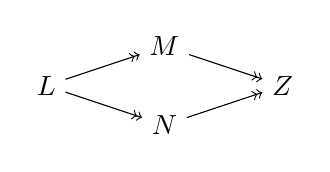
\begin{tikzpicture}
            \node (L) at (0, 0) {$L$};
            \node (M) at (1.5, 0.5) {$M$};
            \node (N) at (1.5, -0.5) {$N$};
            \node (Z) at (3, 0) {$Z$};

            \draw[->>] (L) -- (M);
            \draw[->>] (L) -- (N);
            \draw[->>] (M) -- (Z);
            \draw[->>] (N) -- (Z);
        \end{tikzpicture}
    \end{figure}
    \noindent We can rewrite this result in terms of $\beta$-equality.
    \begin{corollary}
        If $M =_\beta N$\sidefootnote{We use the equality symbol $=_\beta$ to denote equality arising from $\beta$-reduction $\twoheadrightarrow_\beta$.}, then there exists a term $Z$ such that $M \twoheadrightarrow Z$ and $N \twoheadrightarrow Z$.
    \end{corollary}
    \noindent Now, we can answer the uniqueness question.
    \begin{corollary}
        Let $M$ be a term.
        \begin{enumerate}
            \item If $M$ has $N$ as $\beta$-nf, then $M \twoheadrightarrow_\beta N$.
            \item If $M$ has $\beta$-nfs $N_1$ and $N_2$, then $N_1 \equiv N_2$.
        \end{enumerate}
    \end{corollary}
    \begin{proof}
        \hspace*{0pt}
        \begin{enumerate}
            \item We know that $M =_\beta N$. So, there exists a term $Z$ such that $M \twoheadrightarrow_\beta Z$ and $N \twoheadrightarrow_\beta Z$. Since $N$ is a $\beta$-nf, it cannot be reduced any further, meaning that $N \equiv Z$. Hence, $M \twoheadrightarrow_\beta N$.
            
            \item We know that $M =_\beta N_1$ and $M =_\beta N_2$. This implies that $N_1 =_\beta N_2$. Hence, there exists a term $Z$ such that $N_1 \twoheadrightarrow_\beta Z$ and $N_2 \twoheadrightarrow_\beta Z$. Since $N_1$ and $N_2$ are nfs, we find that $N_1 \equiv Z$ and $N_2 \equiv Z$. By transitivity, it follows that $N_1 \equiv N_2$.
        \end{enumerate}
    \end{proof}
    \noindent The first result tells us that there is a reduction sequence that reduces $M$ to its normal form. We are yet to find how this happens; we will come back to that question. The second result tells us that the $\beta$-nf is unique.

    We now prove the Church-Rosser Theorem. To do so, we will define some new concepts, starting with the diamond relation.
    \begin{definition}
        Let $\vartriangleright$ be a binary relation on $\lambda$-terms. We say that the relation $\vartriangleright$ satisfies the \emph{diamond property}, denoted $\vartriangleright {\vDash \diamond}$, if for terms $M, M_1, M_2$,
        \[M \vartriangleright M_1, M \vartriangleright M_2 \implies \exists M_3 . (M_1 \vartriangleright M_3 \land M_2 \vartriangleright M_3).\]
    \end{definition}
    \noindent We will later set $\vartriangleright$ to be the reduction relation, which will allow us to conclude the Church-Rosser. Recall that the transitive closure of a relation is defined as follows:
    \[\frac{}{M \vartriangleright^* M} \qquad \frac{M \vartriangleright N}{M \vartriangleright^* N} \qquad \frac{M \vartriangleright^* N \quad N \vartriangleright^* O}{M \vartriangleright^* O}\]
    We can apply this to the transitive closure of the relation as well. 
    \begin{proposition}
        Let $\vartriangleright$ be a binary relation on $\lambda$-terms such that $\vartriangleright {\vDash \diamond}$. Then, the transitive closure $\vartriangleright^* {\vDash \diamond}$ as well.
    \end{proposition}

    We will now connect the diamond to reduction types (e.g. $\to_\beta$, $\twoheadrightarrow_\beta$, etc.).
    \begin{definition}
        Let $R$ be a definition of reduction. We say that $R$ is \emph{Church-Rosser} if $\twoheadrightarrow_R {\vDash \diamond}$.
    \end{definition}
    We can define equality for a reduction $R$ by extending it to an equivalence relation:
    \[\frac{M \twoheadrightarrow_R N}{M =_R N} \qquad \frac{M =_R N}{N =_R M} \qquad \frac{M =_R N \quad N =_R L}{M =_R L}\]
    \noindent We can prove Church-Rosser theorem for the relations that satisfy the Church-Rosser property.
    \begin{theorem}
        Let $R$ be Church-Rosser. If $M =_R N$, then there exists a term $Z$ such that $M \twoheadrightarrow_R Z$ and $N \twoheadrightarrow_R Z$.
    \end{theorem}
    \begin{proof}
        We show this using structural induction on $M =_R N$. 
        \begin{itemize}
            \item First, assume that $M =_R N$ since $M \twoheadrightarrow_R N$. Then, we can take $Z \equiv N$.
            
            \item Now, assume that $M =_R N$ since $N =_R M$. By the inductive hypothesis, we can find a term $Z$ such that $N \twoheadrightarrow_R Z$ and $M \twoheadrightarrow_R Z$. So, the result holds in this case as well.
            
            \item Finally, assume that $M =_R N$ since $M =_R L$ and $L =_R N$. By the inductive hypothesis, we can find terms $Z_1, Z_2$ such that $M \twoheadrightarrow_R Z_1$, $L \twoheadrightarrow_R Z_1$, $L \twoheadrightarrow_R Z_2$ and $N \twoheadrightarrow_R L$. Since $R$ is Church-Rosser, we know that there exists a term $Z$ such that $Z_1 \twoheadrightarrow_R Z$ and $Z_2 \twoheadrightarrow_R Z$. Since $\twoheadrightarrow_R$ is transitive, we find that $M \twoheadrightarrow_R Z$ and $N \twoheadrightarrow_R Z$. This is summarised in the figure below:
            \begin{figure}[H]
                \centering
                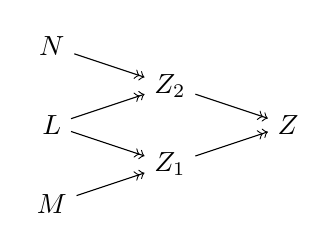
\begin{tikzpicture}
                    \node (N) at (0, 0) {$N$};
                    \node (L) at (0, -1) {$L$};
                    \node (M) at (0, -2) {$M$};
                    \node (Z1) at (1.5, -1.5) {$Z_1$};
                    \node (Z2) at (1.5, -0.5) {$Z_2$};
                    \node (Z) at (3, -1) {$Z$};

                    \draw[->>] (N) -- (Z2);
                    \draw[->>] (L) -- (Z2);
                    \draw[->>] (L) -- (Z1);
                    \draw[->>] (M) -- (Z1);
                    \draw[->>] (Z1) -- (Z);
                    \draw[->>] (Z2) -- (Z);
                \end{tikzpicture}
            \end{figure}
        \end{itemize}
    \end{proof}

    Now, we want to show that $\twoheadrightarrow_\beta$ is Church-Rosser. We would like to do this by showing that $\to_\beta$ is Church-Rosser, but that does not hold. So, we have to define another reduction relation that is more powerful than $\to_\beta$, but its transitive closure is still $\twoheadrightarrow_\beta$. This is the grand reduction.
    \begin{definition}
        The \emph{grand reduction} $\twoheadrightarrow_1$ is defined by the following inference rules:
        \[\frac{}{M \twoheadrightarrow_1 M} \qquad \frac{M \twoheadrightarrow_1 M'}{\lambda x.M \twoheadrightarrow_1 \lambda x.M'}\]
        \[\frac{M \twoheadrightarrow_1 M' \quad N \twoheadrightarrow_1 N'}{MN \twoheadrightarrow_1 M'N'} \qquad \frac{M \twoheadrightarrow_1 M' \quad N \twoheadrightarrow_1 N'}{(\lambda x.M)N \twoheadrightarrow_1 M'[x := N']}\]
    \end{definition}

    We now show that grand reduction subsumes normal reduction.
    % TODO: Make use of inference rules directly (in all structural induction proofs)!
    \begin{proposition}
        Let $M$ and $N$ be terms such that $M \to_\beta N$. Then, $M \twoheadrightarrow_1 N$.
    \end{proposition}
    \begin{proof}
        We prove using structural induction on $M \to_\beta N$.
        \begin{itemize}
            \item First, assume that $M \equiv (\lambda x.A)B$ and $N \equiv A[x := B]$. We have $A \twoheadrightarrow_1 A$ and $B \twoheadrightarrow_1 B$. Hence, $M \equiv (\lambda x.A)B \twoheadrightarrow_1 A[x := B] \equiv N$.
            
            \item Now, assume that $M \equiv \lambda x.M'$ and $N \equiv \lambda x.N'$, with $M' \to_\beta N'$. By inductive hypothesis, we have $M' \twoheadrightarrow_1 N'$. Hence, 
            \[M \equiv \lambda x.M' \twoheadrightarrow_1 \lambda x.N' \equiv N.\]

            \item Next, assume that $M \equiv M'Z$ and $N \equiv N'Z$, where $M' \to_\beta N'$. By inductive hypothesis, we have $M' \twoheadrightarrow_1 N'$. Since we also have $Z \twoheadrightarrow_1 Z$, 
            \[M \equiv M'Z \twoheadrightarrow_1 N'Z \equiv N.\]

            \item Finally, assume that $M \equiv ZM'$ and $N \equiv ZN'$, where $M' \to_\beta N'$. By inductive hypothesis, we have $M' \twoheadrightarrow_1 N'$. Since we also have $Z \twoheadrightarrow_1 Z$,
            \[M \equiv ZM' \twoheadrightarrow_1 ZN' \equiv N.\]
        \end{itemize}
        So, the result follows from induction.
    \end{proof}

    We will now prove some properties of grand reduction that we need to show that grand reduction has the diamond property.
    \begin{proposition}
        Let $M, N, N'$ be terms such that $N \twoheadrightarrow_1 N'$. Then, $M[x := N] \twoheadrightarrow_1 M[x := N']$.
    \end{proposition}
    \begin{proof}
        We prove using structural induction on $M$.
        \begin{itemize}
            \item If $M \equiv x$, then we have
            \[M[x := N] \equiv N \twoheadrightarrow_1 N' \equiv M[x := N'].\]

            \item If $M \equiv y$, where $x$ and $y$ are distinct, then we have
            \[M[x := N] \equiv y \equiv M[x:= N'].\]
            Since $y \twoheadrightarrow_1 y$, we find that $M[x := N] \twoheadrightarrow_1 M[x := N']$.

            \item Now, assume that $M \equiv \lambda y.M'$. The inductive hypothesis tells us that $M'[x := N] \twoheadrightarrow_1 M'[x := N']$. Hence, 
            \[M[x := N] \equiv (\lambda y.M' [x := N]) \twoheadrightarrow_1 (\lambda y.M' [x := N']) \equiv M [x := N'].\]

            \item Finally, assume that $M \equiv KL$. The inductive hypothesis tells us that $K[x := N] \twoheadrightarrow_1 K[x := N']$ and $L[x := N] \twoheadrightarrow_1 L[x := N']$. So,
            \[M[x:= N] \equiv K[x := N] L[x := N] \twoheadrightarrow_1 K[x := N'] L[x := N'] \equiv M[x := N'].\]
        \end{itemize}
        So, the result follows from induction.
    \end{proof}

    \begin{proposition}
        Let $M, M', N, N'$ be terms such that $M \twoheadrightarrow_1 M'$ and $N \twoheadrightarrow_1 N'$. Then, $M[x := N] \twoheadrightarrow_1 M'[x := N']$.
    \end{proposition}
    \begin{proof}
        We prove using structural induction on $M \twoheadrightarrow_1 M'$.
        \begin{itemize}
            \item If $M \equiv M'$, then we have
            \[M[x := N] \twoheadrightarrow_1 M[x := N'] \equiv M'[x := N].\]

            \item Now, assume that $M \equiv \lambda y.L$ and $M' \equiv \lambda y.L'$. By inductive hypothesis, we know that $L[x := N] \twoheadrightarrow_1 L'[x := N']$. Hence,
            \begin{align*}
                M[x := N] &\equiv \lambda y.L[x := N] \\
                &\twoheadrightarrow_1 \lambda y.L'[x := N'] \\
                &\equiv M'[x := N'].
            \end{align*}

            \item Next, assume that $M \equiv KL$ and $M' \equiv K'L'$. By inductive hypothesis, we know that $K[x := N] \twoheadrightarrow_1 K'[x := N']$ and $L[x := N] \twoheadrightarrow_1 L'[x := N']$. Hence,
            \begin{align*}
                M[x := N] &\equiv K[x := N] L[x := N] \\
                &\twoheadrightarrow_1 K'[x := N'] L'[x := N'] \\
                &\equiv M'[x := N'].
            \end{align*}

            \item Finally, assume that $M \equiv (\lambda y.K)L$ and $M' \equiv K'[y := L']$. By inductive hypothesis, we know that $K[x := N] \twoheadrightarrow_1 K'[x := N']$ and $L[x := N] \twoheadrightarrow_1 L'[x := N']$. Hence,
            \begin{align*}
                M[x := N] &\equiv (\lambda y.K[x := N])L[x := N] \\
                &\twoheadrightarrow_1 (\lambda y.K'[x := N'])L'[x := N'] \\
                &\equiv M'[x := N'].
            \end{align*}
        \end{itemize}
        So, the result follows from induction.
    \end{proof}

    \begin{proposition}
        Let $M$ and $N$ be terms with $\lambda x.M \twoheadrightarrow_1 N$. Then, there exists a term $M'$ such that $N \equiv \lambda x.M'$ with $M \twoheadrightarrow_1 M'$.
    \end{proposition}
    \begin{proof}
        We show this by considering the cases of $\twoheadrightarrow_1$:
        \begin{itemize}
            \item First, assume that $N \equiv \lambda x.M$. The result holds since $M \twoheadrightarrow_1 M$.
            \item Now, assume that $N \equiv \lambda x.M'$, where $M \twoheadrightarrow_1 M'$. Here as well, the result holds.
        \end{itemize}
    \end{proof}

    \begin{proposition}
        Let $M, N, L$ be terms such that $MN \twoheadrightarrow_1 L$. Then, either
        \begin{enumerate}
            \item $L \equiv M' N'$ with $M \twoheadrightarrow_1 M'$ and $N \twoheadrightarrow_1 N'$ or
            \item $M \equiv \lambda x.P$ and $L \equiv P'[x := N']$, with $P \twoheadrightarrow_1 P'$ and $N \twoheadrightarrow_1 N'$.
        \end{enumerate}
    \end{proposition}
    \begin{proof}
        We show this by considering the cases of $\twoheadrightarrow_1$:
        \begin{itemize}
            \item First, assume that $L \equiv MN$. Since $M \twoheadrightarrow_1 M$ and $N \twoheadrightarrow_1 N$, case (1) holds.
            \item Next, assume that $L \equiv M'N'$, where $M \twoheadrightarrow_1 M'$ and $N \twoheadrightarrow_1 N'$. Clearly, case (1) holds.
            \item Finally, assume that $M \equiv \lambda x.P$, and $L \equiv P'[x := N']$, with $P \twoheadrightarrow_1 P'$ and $N \twoheadrightarrow_1 N'$. Clearly, case (2) holds in this case.
        \end{itemize}
    \end{proof}

    \begin{proposition}
        The relation $\twoheadrightarrow_1$ has the diamond property, i.e. for terms $M, M_1, M_2$,
        \[M \twoheadrightarrow_1 M_1, M \twoheadrightarrow_1 M_2 \implies \exists M_3 . (M_1 \twoheadrightarrow_ 1 M_3, M_2 \twoheadrightarrow_1 M_3).\]
    \end{proposition}
    \begin{proof}
        We show this by induction on $M$.
        \begin{itemize}
            \item First, assume that $M \equiv x$, where $x$ is a variable. Since $x$ is a normal form, it follows that $M_1 \equiv x$ and $M_2 \equiv x$. Hence, set $M_3 \equiv x$, and the result follows.

            \item Now, assume that $M \equiv \lambda x.M'$. By the result above, it follows that $M_1 \equiv \lambda x.N_1$ and $M_2 \equiv \lambda x.N_2$, where $M' \twoheadrightarrow_1 N_1$ and $M' \twoheadrightarrow_1 N_2$. So, the inductive hypothesis tells us that there exists an $N'$ such that $N_1 \twoheadrightarrow_1 N'$ and $N_2 \twoheadrightarrow_1 N'$. Hence, set $M_3 \equiv \lambda x.N'$, and the result follows.
            
            \item Finally, assume that $M \equiv PQ$. By the result above, we know that there are 2 choices here:
            \begin{itemize}
                \item First, let $M_1 \equiv P_1 Q_1$ and $M_2 \equiv P_2 Q_2$, where $P \twoheadrightarrow_1 P_1, P \twoheadrightarrow_2 P_2$, and $Q \twoheadrightarrow_1 Q_1, Q \twoheadrightarrow_2 Q_2$. By the inductive hypothesis, there exist $P'$ and $Q'$ such that $P_1 \twoheadrightarrow_1 P', P_2 \twoheadrightarrow_1 P'$ and $Q_1 \twoheadrightarrow_1 Q', Q_2 \twoheadrightarrow_1 Q'$. Hence, set $M_3 \equiv P' Q'$.
                
                \item Otherwise, we have $P \equiv \lambda x.P'$ and $M_1 \equiv P'[x := Q_1]$, where $Q \twoheadrightarrow_1 Q_1$. Hence, we must also have $M_2 \equiv P'[x := Q_2]$, where $Q \twoheadrightarrow_1 Q_2$. By the inductive hypothesis, there exists a $Q$ such that $Q_1 \twoheadrightarrow_1 Q$ and $Q_2 \twoheadrightarrow_1 Q'$. Hence, set $M_3 \equiv \lambda x.Q$.
            \end{itemize}
        \end{itemize}
    \end{proof}

    \begin{theorem}
        The transitive closure of the relation $\twoheadrightarrow_1$ is $\twoheadrightarrow_\beta$.
    \end{theorem}
    \noindent Now, we have shown that $\beta$-reduction satisfies the Church-Rosser, and hence the Church-Rosser Theorem holds. That is,
    \begin{itemize}
        \item $\beta$-nfs are unique, and
        \item if a term has a $\beta$-nf, then it is possible to reduce the term to that normal form.
    \end{itemize}
    This also allows us to prove that the $\lambda$-theory is consistent. If $M$ and $N$ are distinct nfs, then we cannot have $M = N$. Otherwise, there would be a term $Z$ that both $M$ and $N$ reduce to by Church-Rosser.

    \subsection{Reduction Strategies}
    We now focus on how to get the normal form.    
    \begin{theorem}[Normalisation Theorem]
        Let $M$ be a term. If it has a normal form, then iterated reductions of the leftmost redex leads to the normal form.
    \end{theorem}
    \noindent The leftmost reduction strategy is therefore \emph{normalising}. It can be used to find the normal form for a term, or to show that a term has no normal form. There are two forms of normalisation:
    \begin{itemize}
        \item \emph{Weak normalisation}, where there exists a path that leads to the normal form, e.g. the factorial function.
        \item \emph{Strong normalisation}, where every path leads to the normal form, e.g. $(\lambda xy. x + y)(1 + 2)(3 + 4)$.
    \end{itemize}

    In $\lambda$-calculus, there are 2 reduction strategies, both of which are leftmost- \emph{call-by-value} and \emph{call-by-need}. A term of the form $\lambda x.M$ is considered a \emph{value}- it is the final result of a computation. Call-by-value uses \emph{leftmost innermost} strategy (and is seen in Python), and call-by-need (or lazy evaluation, in Haskell) uses \emph{leftmost outermost} strategy:
    \begin{itemize}
        \item By leftmost, we mean that in an application $MN$, $M$ is reduced first, and then $N$.
        \item By innermost, we mean that in the term $(\lambda x.M) N$, $N$ is reduced to a value before $M[x := N]$ is computed.
        \item By outermost, we mean that in the term $(\lambda x.M) N$, $M[x := N]$ is reduced to a value before $N$ is computed. 
    \end{itemize}
    In leftmost outermost strategy, we might have to compute $N$ multiple times. To avoid this, we can compute it first, and then use the same value for other occurrences of $N$. If expressions do not have side-effects, then this produces the same result as a pure leftmost outermost strategy, where $N$ is evaluated every time it appears.
    \newpage

    \section{Computability}
    In this section, we consider \emph{computability}. Computability requires a definition of computation. There are many notions of computation, including $\lambda$-calculus, automata and register machines. They all capture the same notion of computability. The \emph{Church-Turing Thesis} states that collectively, these definitions are the `true' notion of computation.

    To formalise computability, we will consider ways of defining functions on positive integers (i.e. natural numbers). We can use $\lambda$-terms to represent natural numbers and booleans, and fixed-point operators to define recursive functions. We will show that recursive functions can be converted into $\lambda$-terms.

    \subsection{Primitive Recursive Functions}
    We show that $\lambda$-calculus is the right model of computation by showing it is equivalent to recursive functions. We start by defining \emph{primitive recursive functions}. They can be defined using a fixed type of \emph{recursive functions}. The primitive recursive functions are functions $\mathbb{N} \times \dots \times \mathbb{N} \to \mathbb{N}$ that can be defined using the following \emph{initial functions}:
    \begin{itemize}
        \item the \emph{constant zero function} 
        \[Z(n) = 0\]
        \item the \emph{successor function} 
        \[S^+(n) = n+1\]
        \item the \emph{selector function} 
        \[U_{i, p}(n_0, \dots, n_p) = n_i\]
        for $0 \leq i \leq p$ and $p \in \mathbb{N}$;
        \item \emph{composition} 
        \[F(\vec{n}) = H(G_1(\vec{n}), \dots, G_m(\vec{n}))\]
        where $H, G_1, \dots$, $G_m$ are primitive recursive functions.
    \end{itemize}
    Now, we say that a function $F$ is \emph{primitive recursive} if it is of the form
    \begin{align*}
        F(0, \vec{n}) &= H(\vec{n}) \\
        F(k+1, \vec{n}) &= G(F(k, \vec{n}), k, \vec{n}),
    \end{align*}
    where $H$ and $G$ are primitive recursive. In other words, 
    \begin{itemize}
        \item $F(0, \vec{n})$ is the \emph{base case}, and only depends on the `other' data $\vec{n}$, and
        \item the \emph{recursive case} $F(k+1, \vec{n})$ depends on the previous result $F(k, \vec{n})$ along with the number $k$ and the data $\vec{n}$.
    \end{itemize}
    We now give examples of functions in primitive recursion:
    \begin{itemize}
        \item the identity function on $\mathbb{N}$ is given by $id(n) = U_{0, 0}(n)$.
        
        \item the addition function is given by
        \begin{align*}
            \operatorname{add}(0, n) &= id(n) \\
            \operatorname{add}(k+1, n) &= G(\operatorname{add}(k, n), k, n),
        \end{align*}
        where $G(x, y, z) = S^+(U_{0, 2}(x, y, z))$, i.e. $G(x, y, z) = x+1$.

        \item the multiplication function is given by
        \begin{align*}
            \operatorname{mult}(0, n) &= Z(n) \\
            \operatorname{mult}(k+1, n) &= G(\operatorname{mult}(k, n), k, n),
        \end{align*}
        where $G(x, y, z) = \operatorname{add}(U_{0, 2}(x, y, z), U_{2, 2}(x, y, z))$, i.e. $G(x, y, z) = x + z$.

        \item the factorial function is given by
        \begin{align*}
            \operatorname{fact}(0) &= S^+(0) \\
            \operatorname{fact}(k+1) &= G(\operatorname{fact}(k), k),
        \end{align*}
        where $G(x, y) = \operatorname{mult}(U_{0, 1}(x, y), S^+(U_{1, 1}(x, y)))$, i.e. $G(x, y) = x * (y+1)$.

        \item the sum of the first $n$ numbers is given by
        \begin{align*}
            \operatorname{sum}(0) &= 0 \\
            \operatorname{sum}(k+1) &= G(\operatorname{sum}(k), k),
        \end{align*}
        where $G(x, y) = \operatorname{add}(U_{0, 1}(x, y), S^+(U_{1, 1}(x, y)))$, i.e. $G(x, y) = x + (y + 1)$.
    \end{itemize}

    \subsection{Recursive functions and minimalisation}
    It turns out that primitive recursion is not the right definition for computability. To see this, consider the following function, called the \emph{Ackermann's function}:
    \begin{align*}
        A(0, n) &= n + 1 \\
        A(m + 1, 0) &= A(m, 1) \\
        A(m+1, n+1) &= A(m, A(m+1, n)).
    \end{align*}
    Because each $m$ or $n$ is decreasing at each step, we know that the computation $A(m, n)$ terminates for every natural number $m$ and $n$. However, the values of this function grow very fast, e.g. $A(4, 2)$ has about 20 000 digits! It turns out that Ackermann's function grows faster than any primitive recursive function, so it cannot be primitive recursive. However, we \emph{were} able to give a recursive definition for it above, so primitive recursion is not the definition of computability we want.

    To define the bigger class of recursive functions, we need one more notion. If $P(n)$ is a predicate on $\mathbb{N}$, i.e. a function $\mathbb{N} \to bool$, then we denote by $\min n[P(n)]$ the smallest number $n$ such that $P(n)$ holds; if there is no such number, then the value is undefined. We say that a function $F$ is \emph{recursive} if it can be defined using primitive recursion and \emph{minimalisation}:
    \[F(\vec{n}) = \min m[H(\vec{n}, m) = 0],\]
    where for any $\vec{n}$, there is a natural number $m$ such that $H(\vec{n}, m) = 0$.

    Intuitively, primitive recursion allows us to write bounded loops, i.e. \textit{for}-loops. In particular, the number of iterations is bounded by a value in the program, i.e. the initial value of the argument. Minimalisation corresponds to a \textit{while}-loop- we continue looping until the predicate becomes \textit{false}. This also gives an intuitive argument as to why recursive functions are a good definition for computable functions. Although not clear, it is possible to write Ackermann's function using primitive recursion and minimalisation.

    Now, we will show that $\lambda$-calculus can be used to write recursive functions. We can define the initial functions as follows:
    \begin{align*}
        U_{i, p} &\equiv \lambda x_0 \dots x_p. x_i \\
        S^+ &\equiv \lambda x.\texttt{pair}(F)(x) \\
        Z &\equiv \lambda x.x
    \end{align*}
    For composition $F(\vec{n}) = H(G_1(\vec{n}, \dots, G_m(\vec{n})))$, we define
    \[F \equiv \lambda \vec{x}.H(G_1\vec{x}) \dots (G_m \vec{x})\]
    Next, let $F$ be a primitive recursive function
    \begin{align*}
        F(0, \vec{n}) &= H(\vec{n}) \\
        F(k+1, \vec{n}) &= G(F(k, \vec{n}), k, \vec{n}),
    \end{align*}
    where $H$ and $G$ are defined by $\lambda$-terms $H$ and $G$. Then, we can define $F$ to be the fixed point of the function $f$:
    \[f \equiv \lambda f x \vec{y}. (\textit{if} \ (\textit{iszero} \ x) \ (H \ \vec{y}) \ (G(f(P\ x) \vec{y}) (P \ x)(\vec{y}))),\]
    where $P$ is the predecessor function.

    Finally, we define minimalisation. To do so, let $P$ be the predicate. We define a function that iterates from a given number $n$ until $P \ n$ is true, and returns $n$. So, it can be the fixed point of the function
    \[h_P \equiv \lambda hz.\textit{if} \ (P \ z) \ (z) \ (h(S^+ \ z)).\]
    So, $\textit{min} P \equiv \texttt{fix}(h_p)(Z)$, where $Z \equiv \lambda x.x$ is zero. If $F$ is given by
    \[F(\vec{n}) = \min m[H(\vec{n}, m) = 0],\]
    where $H$ is defined by a $\lambda$-term $H$, then we can define $F$ by
    \[F \equiv \lambda \vec{x}.\textit{min} \ (\lambda y.\textit{iszero} \ H \ \vec{x} \ y).\]
    Hence, every recursion function can be defined in $\lambda$-calculus. This means that $\lambda$-calculus is sufficient for general recursion and can be used to extend primitive recursion instead of minimalisation.

    It is also true that every function $\mathbb{N} \times \dots \times \mathbb{N} \to \mathbb{N}$ that we can defined in $\lambda$-calculus can be defined in $\lambda$-calculus. To do so, we can encode $\lambda$-terms as numbers and define reduction as a function.
    \newpage

    \section{Simply-typed $\lambda$-calculus}
    In this section, we introduce type checking for $\lambda$-calculus. We have presented $\lambda$-calculus as a foundation for functional programming, and shown how to represent data and define interesting functions. Many standard programming languages have static or compile-time type-checking. The types we add to $\lambda$-calculus give rise to \emph{simply-typed $\lambda$-calculus}, where simply refers to the fact that this is the simplest of its kind and we can build on it in many ways, e.g. by adding polymorphism.

    Initially, we will not give concrete types such as \textit{int} or \textit{bool}. We will instead start with some type $A$, using which we define functions. Hence, types are defined by the following BNF rule:
    \begin{align*}
        T &::= A \\
        &| \hspace*{10pt} T \to T
    \end{align*}
    So, some types are $A$, $A \to A$ and $(A \to A) \to (A \to A)$. By convention, the arrow operation $\to$ is right-associative, meaning that the final type can be written as $(A \to A) \to A \to A$.

    In $\lambda$-terms, we have bound and free variables. The bound variables have a fixed type that can be stated within the $\lambda$-term. This is similar to many programming languages, where the arguments are given with their types. But, for us to keep track of the types of free variables, we keep use of a \emph{typing context}. A typing context $\Gamma$ is a set of variables associated to types, and defined by the following BNF:
    \begin{align*}
        \Gamma &::= \varnothing \\
        &| \hspace*{10pt} \Gamma, x \colon T.
    \end{align*}
    The first rule presents a context with no variables. In the second rule $\Gamma, x \colon T$, we have extended an existing typing context $\Gamma$ with a new variable-type pair: $x \colon T$.

    Now, let $\Gamma$ be a typing context and $M$ a term. If the term $M$ has type $T$ under the typing context $\Gamma$, then we denote this by $\Gamma \vdash M \colon T$. This is called \emph{typing judgment}. We introduce a variation on the syntax for bounded variables, i.e. $\lambda x \colon T.M$, which means that $x$ has type $T$. This is a \emph{Church-style definition}.

    We now define typing rules using inference rules:
    \[\frac{x \colon T \in \Gamma}{\Gamma \vdash x \colon T}\textrm{TVar} \] 
    Note that this is an axiom, i.e. $x \colon T \in \Gamma$ is a side condition. The TVar rule states that if the typing context $\Gamma$ contains the rule $x \colon T$, then under $\Gamma$, $x$ has type $T$. 
    \[\frac{\Gamma, x \colon T \vdash M \colon U}{\Gamma \vdash \lambda x \colon T.M \colon T \to U} \textrm{TAbs}\]
    The TAbs rule extends a typing context to an abstraction. In particular, if under $\Gamma$ and $x \colon T$, $M$ has type $U$, then the abstraction $\lambda x \colon T. M$ has type $T \to U$ under $\Gamma$. We make use of a comma to denote union of typing contexts.    
    \[\frac{\Gamma \vdash M \colon T \to U \quad \Gamma \vdash N \colon T}{\Gamma \vdash MN \colon U} \textrm{TApp}\]
    Like with abstraction, we have the TApp rule for application. In this case, if we have $M$ of type $T \to U$ and $N$ of type $T$, then $MN$ has type $U$.

    We will now consider some typing derivations for $\lambda$-terms. We start with the term $\lambda x.x$:
    \[\nfrac{\nfrac{x \colon A \in x \colon A}{x \colon A \vdash x \colon A} \textrm{TVar}}{\vdash \lambda x \colon A. x \colon A \to A} \textrm{TAbs}\]
    In this case, the typing context is empty, and is denoted by nothing to the left of $\vdash$. We typically do not keep the TVar applications in the inference rules. Next, we do the typing derivation for $\lambda xy.x$:
    \[\nfrac{\nfrac{x \colon A, y \colon A \vdash x \colon A}{x \colon A \vdash \lambda y \colon A.x \colon A \to A} \textrm{TAbs}}{\vdash \lambda x \colon A.\lambda y \colon A.x \colon A \to A \to A}\textrm{TAbs} \]

    We now add some concrete rules in all typing judgments. We start by adding some axioms:
    \[\frac{}{\Gamma \vdash \textit{true} \colon \textit{bool}} \textrm{TTrue} \quad \frac{}{\Gamma \vdash \textit{false} \colon \textit{bool}} \textrm{TFalse} \quad \frac{v \textrm{ is an integer literal}}{\Gamma \vdash v \colon \textit{int}} \textrm{TInt}\]
    Next, we add some mathematical operations and conditions.
    \[\frac{\Gamma \vdash M \colon \textit{bool} \quad \Gamma \vdash N \colon \textit{bool}}{\Gamma \vdash M \textrm{ and } N \colon \textit{bool}} \textrm{TAnd} \qquad \frac{\Gamma \vdash M \colon \textit{int} \quad \Gamma \vdash N \colon \textit{int}}{\Gamma \vdash M + N \colon \textit{int}} \textrm{TPlus}\]
    \[\frac{\Gamma \vdash M \colon \textit{int} \quad \Gamma \vdash N \colon \textit{int}}{\Gamma \vdash M == N \colon \textit{bool}} \textrm{TEq}\]
    \[\frac{\Gamma \vdash L \colon \textit{bool} \quad \Gamma \vdash M \colon T \quad \Gamma \vdash N \colon T}{\Gamma \vdash \texttt{if } L \texttt{ then } M \texttt{ else } N \colon T} \textrm{TCond}\]
    These allow us to do mathematical reductions and ensure that we still have a type to assign to the result.

    We will now show that well-typed programs do not go wrong. The point of introducing a static (compile-time) type system is that type checking guarantees the absence of runtime type errors. To show this, we first need to define wrong programs. This is achieved by adding the special term \textit{wrong} to the syntax of $\lambda$-terms, and modify the reduction rules, e.g. 
    \[1 + \textit{true} \to_\beta \textit{wrong}.\] 
    This term models stuck computations that are not values.

    To show that well-type programs don't go wrong, we require the \emph{Type Safety Theorem}. This is given in two parts- \emph{type preservation} and \emph{progress}.
    \begin{theorem}[Type Preservation]
        If $\Gamma \vdash M \colon T$ and $M \to_\beta N$, then $\Gamma \vdash N \colon T$.
    \end{theorem}
    \begin{theorem}[Progress]
        If $\Gamma \vdash M \colon T$, then either $M$ is a value or there exists $M'$ such that $M \to_\beta M'$.
    \end{theorem}
    \noindent We say that the term \textit{wrong} is untypeable, i.e. if $\Gamma \vdash M \colon T$, then we cannot have $M \twoheadrightarrow_\beta \textit{wrong}$.

    Unfortunately, simply-typed $\lambda$-calculus does not support recursion. This is because any $\operatorname{fix}$ term isn't typeable. For instance, consider the following
    \[\operatorname{fix} = \lambda f.(\lambda y.f(\lambda z.yyz))(\lambda y.f(\lambda z.yyz))\]
    The term $yyz$ is not typeable since that implies $y$ is of the form $A \to A \to A$ and $A$ at the same time. Hence, we recursive functions are not well-typed.

    So, in a typed functional programming, we have to add a built-in construct, by either adding the $\operatorname{fix}$ term to have type
    \[\operatorname{fix} \colon (T \to T) \to T\]
    for every type $T$, or by supporting recursive functions, e.g.
    \[\operatorname{fac}(n \colon \textit{int}) \colon \textit{int} = \textit{if } n == 0 \textit{ then } 1 \textit{ else } n * \operatorname{fac}(n-1).\]
    Adding recursion this way maintains the property that well-typed programs do not contain runtime type errors.

    The simply-typed $\lambda$-calculus has an important property of \emph{strong normalisation}. This means that every typeable term has a normal form, which can be reached by $\beta$-reduction. Because of the Church-Rosser Theorem, it doesn't matter which reduction strategy is used; we no longer have to worry about non-termination, so any strategy will eventually produce the unique normal form of a term. This is another way to see why fix is untypeable- if we could type fix, then we would be able to define recursive functions that fail to terminate, which contradicts the strong normalisation property.

    It is possible to implement an algorithm to check whether or not a given term is typeable (\emph{type inference}), and to check whether or not a given term has a given type (\emph{type checking}). Typeability and type checking are different problems- the typeability problem is solved by a type inference algorithm and finds the most general type of a given term, if typeable. Type inference is used in Haskell.

    Now, we consider the expressivity of simply-typed $\lambda$-calculus. We know that $\lambda$-calculus is able to express all computations, but this required the construction of recursive functions. Since simply-typed $\lambda$-calculus does not allow recursion, it is not Turing-complete. We can add recursion in a type-safe manner to give us a typed programming language that is Turing-complete.
    
\end{document}